\scanpage{100}
% archive sheet number: 102

\uline{Cor} Supposons $k$ principal, \inserted{$2$-régulier} $k_0=k/2k$ un corps. Alors les \inserted{\unsure{cl. d'isom|cl. de tels|à isom. près}} $(M,\sigma)$ précédents reviennent à : celles des paires $(P,Q,\deleted{\unsure{p,q,m|p,q}})$ avec $P,Q$ libres de rang $1$, et \deleted{\unsure{$p\,q$|$p$|$p\subset$}} $m\subset\underbrace{P/\unsure{2|k}P}_{p}\oplus\underbrace{Q/2Q}_{q}$ sous-esp. vectoriel sur $k_0$, \deleted{\unsure{de tel que|du tel que}} qui est soit nul, soit une droite $\ne p,q$ (droites coordonnées)

\uline{Cor} Cela donne une classification des classes de conjugaison d'éléments de $\mathrm{Gl}(2,k)\deleted{\unsure{^*|^-}}$ qui sont d'ordre $2$ exactement, et distincts de $\{\pm1\}$ : il y \deleted{en a} a \inserted{celle de} $\left(\begin{smallmatrix}1&0\\0&-1\end{smallmatrix}\right)$ (correspondant au cas $m=0$), puis \uline{une} \deleted{\unsure{famille entière|famille indexée|familles indexées} par l'ens des \unsure{points|gens} de $\mathbf P^1(k_0)$ distincts de $0,\infty$ (en supposant que $k^*\to k_0^*$ est surjectif, sinon la classification sera plus fine,} \inserted{en supposant que $k^*\to k_0^*$ surj, on} peut via des bases de $P/2P$ resp. $Q/2Q$ se ramenant à une base de $P,Q$.

Elle correspond à

\[
\begin{aligned}
&P=k,\ Q=k,\ m=\text{diagonale de }k_0\times k_0\quad\text{i.e.}\\
&M'=(2k\oplus2k)+\operatorname{diag.}\text{ de }k\oplus k=\{(x,y)\mid x-y\in2k\}
\end{aligned}
\]

donc on peut prendre base de $M'$

\[
\unsure{u|e_u|u_0}=(2,0),\quad\unsure{v|e_v|v_1}=(1,1),\quad\text{d'où}\quad -u+2v=(0,2)=\text{sym}(u)
\]

\margin{$u=2e_0$\\ $v=e_0+e_1$}

On trouve

\[
\sigma u=u,\quad \sigma v\ \deleted{\unsure{\ne|+|=}}(1,-1)=u-\mathrm{sym}\,v=u-v
\]

i.e. la matrice de $\sigma$ p. r. à $(u,v)$ est

\[
\begin{pmatrix}1&1\\0&-1\end{pmatrix}
\]

Dans le cas de $k=\mathbb Z$, c'est la matrice de la réflexion p. r. à la diagonale $0,e_0$ de l'hexagone régulier, la fig. de l'hexagone étant rapporté à un syst. de coordonnées obliques ayant comme base deux sommets consécutifs $u,v$ ($M$ est le réseau engendré par l'un des sommets).

\figure{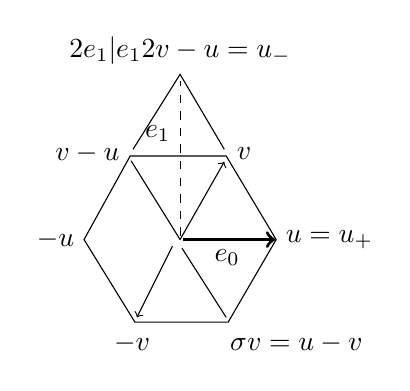
\begin{tikzpicture}[x=1.22cm,y=1.22cm]
\draw (-1,0)--(-.52,.87)--(.48,.87)--(1,0)--(.50,-.86)--(-.47,-.86)--cycle;
\draw (-.49,.94)--(0,1.72)--(.46,.94);
\draw[->] (0,0)--(.46,.81);\draw[->,very thick] (.03,0)--(.99,0);\draw[->] (-.08,-.07)--(-.45,-.81);\draw (0,0)--(-.51,.82) (.02,-.09)--(.48,-.81);
\draw[dashed] (0,.04)--(0,1.65);
\node[above] at (0,1.72) {$\deleted{\unsure{2e_1|e_1}}2v-u=u_-$};\node[left] at (-.53,.9) {$v-u$};\node[right] at (.49,.90) {$v$};\node[left] at (-1,0) {$-u$};\node[left] at (0,1.1) {$e_1$};\node[below] at (.49,0) {$e_0$};\node[right] at (1,0) {$u=u_+$};\node[below] at (-.50,-.88) {$-v$};\node[below right] at (.42,-.89) {$\sigma v=u-v$};
\end{tikzpicture}}

\margin{\uline{NB} Soit $u_+$ une base de $\pi_+$, $u_-$ une base de $\pi_-$, alors \deleted{dans} On peut représenter $\sigma_{\mathbb R}$, pour la base $(u_+,u_-)$ de $\pi\otimes_{\mathbb Z}\mathbb R$ par la matrice $\left(\begin{smallmatrix}1&0\\0&-1\end{smallmatrix}\right)$ le réseau $\pi$ étant identifié à $\mathbb Zu_-+\mathbb Zu_+$ \inserted{$\simeq\mathbb Z^2$} dans le premier cas, et dans le $2^{\text{ème}}$ à l'ens des $\unsure{x|a}u_++yu_-$ tels que $x-y\in\mathbb Z$, $x,y\in\frac12\mathbb Z$}

\margin{$\sigma^2(e_1)=\sigma e_0-\sigma e_1=e_0-(e_0-e_1)=e_1$}
